\section{Behandlingsforløb}
\textit{I dette afsnit beskrives behandlingsforløbet for knæartrosepatienter, herunder de forskellige behandlingsmetoder, der kan anvendes. Non-invasive behandlingsmetoder undersøges for at bestemme effekten af disse, hvorefter anvendelsen af invasive behandlingsmetoder samt kriterierne for et succesfuldt kirurgisk indgreb analyseres med henblik på at vurdere, om operationsteknikken er årsag til, at patienter udvikler kroniske postoperative smerter.}

Behandlingsforløbet for en patient med knæartrose består af flere behandlingsmetoder. Målet med behandling af knæartrose er smertelindring, mobilitetsforøgelse samt forebyggelse. Generelt kan metoderne inddeles i non-invasive og invasive. Behandlingsvalget afhænger af sygdommens omfang. \citep{Lind2016b} Et flowchart over behandlingsforløbet for en artrosepatient ses på \figref{fig:flow_behandlingsfaser}. 

\begin{figure}[H]
	\centering
	\includegraphics[width=1\textwidth]{figures/bProblemanalyse/flowchart_behandlingsforloeb_rettet.png}
	\caption{Figuren illustrerer et flowchart der viser de forskellige behandlingsmetoder, en patient med knæartrose gennemgår. Livsstilsændring dækker eksempelvis vægtreduktion, mens medicinsk behandling er smertelindrende stoffer og kirurgiske indgreb er eksempelvis alloplastikker. \citep{Lind2016b}}
	\label{fig:flow_behandlingsfaser}
\end{figure}\vspace{-.25cm}

%Ved en sådan overvejelse vurderes den diagnosticerede grad af artrose, ud fra den kliniske vurdering og forandringer i knæet fundet ved røntgenbilleder. Både de kliniske observationer og røntgenbilleder anvendes som vurderingsgrundlag idet smerte fra hofte og ryg kan projiceres til knæet. Hermed tilbydes patienten først en TKA-operation, når non-invasive behandlingsmetoder ikke har lindret symptomer i en tilstrækkelig grad. \citep{brostrom2012}

\subsection{Non-invasiv behandling}
Artrose kan ikke helbredes og non-invasive behandlingsmetoder vil derfor fortrinsvis søge at smertelindre samt forbedre mobiliteten af knæleddet. En essentiel del af behandlingen består i at informere og uddanne patienten, give indsigt i sygdommen samt at inddrage patienten i behandlingsforløbet. \citep{brostrom2012} Som det ses på \figref{fig:flow_behandlingsfaser}, består første fase i den non-invasive behandling af en livsstilsændring, hvor en vægtreduktion samt øget fysisk aktivitet forsøges for at afhjælpe patientens symptomer. Hvis dette ikke er tilstrækkeligt, kan medicinsk behandling i form af smertelindrende medikamenter benyttes, enten som enkeltstående behandling eller sideløbende med fysioterapi, der har til formål at styrke muskulaturen omkring leddet.
De benyttede medikamenter er paracetamol, men også non steroidal anti-inflammatory drug (NSAID) præparater kan anvendes ved inflammation \citep{schroder}. Ved kraftige smertegener, hvor de primære præparater til behandling ikke har haft den ønskede effekt, kan opioider benyttes. \citep{brostrom2012}\\
I både nationale og internationale kliniske retningslinjer, er der bred konsensus om, at træning er af væsentlig betydning ved behandling af knæartrose \citep{brostrom2012}. Et studie med data fra over 4.000 patienter, foretaget af \citer{Syssorenskou} viste, at hverken graden af den radiologiske artrose eller smerteintensitet havde indvirkning på hvor stor effekt, der kunne forventes af træningsforløbet. Det blev fundet, at patienter med svær artrose oplevede samme smertereduktion, som patienter med let til moderat artrose. Et studie af \citer{sorenskou} fandt evidens for, at smertelindringen ved træning var lige så stor som ved brug af NSAID'er og endnu større end ved brug af paracetamol. Træning har desuden, modsat medicinsk behandling, ingen bivirkninger. \citep{sorenskou}
Et studie af \citer{newEngland} fulgte 100 knæartrosepatienters behandlingsforløb over et år. Den ene gruppe modtog non-invasiv behandling, som bestod af et træningsforløb, patientundervisning, indlægssåler og et eventuelt vægttabsprogram. Den anden gruppe modtog kirurgisk behandling. Gruppen, der gennemgik kirurgisk behandling, havde en større smertelindring end gruppen, som kun modtog non-invasiv behandling. Gruppen der modtog kirurgisk behandling, havde imidlertid større risiko for at få svære komplikationer. Forsøget viste dog, at i gruppen som modtog non-invasiv behandling, fik omkring en tredjedel foretaget en TKA-operation i løbet af forsøgsperioden. \citep{newEngland} Herudfra er der indikationer for, at non-invasiv behandling er en effektiv metode til behandling af knæartrose, og kan anvendes som metode til at udskyde behovet for et invasivt indgreb. Det antydes imidlertid ligeledes, at invasiv behandling stadig vil være nødvendigt. 

%Dette kan muligvis betyde at et non-invasivt forløb kan være være med til udskyde et operativt indgreb. (\textbf{vi skal nok passe på med at konkludere noget her})

%\subsection{Knæartrose}
%
%Knæartrose også kaldet slidgigt i knæene, har mange årsager. Hvor af nogle er overvægt, arv, traume eller tungt arbejde. Arterose er karakteriseret ved ødelæggelse af ledbrusken med dertil hørende reaktioner i de tillæggende knogler og slimhinder. Symptomerne på knæartrose er smerte, funktionstab og fejlstilling, hvilket besværliggøre hverdagen. 
%Ved knæartrose er sidste behandlings skridt kirurgi, afhængig af graden af traumet er forskellige kirurgiske indgreb en mulighed. [Nationale retningslinjer] 

\subsection{Invasiv behandling} \label{kirurgiskbehandling}
Som det fremgår af \figref{fig:flow_behandlingsfaser} er invasiv behandling det sidste trin i behandlingsforløbet for en patient med knæartrose. Invasive behandlingsmetoder kan anvendes, når de non-invasive behandlingsmetoder ikke længere afhjælper lidelsen i en grad hvor patienten er tilfreds. Som invasiv behandling for knæartrose foretages oftest en alloplastik. En alloplastik er et kirurgisk, der har til formål helt eller delvist at udskifte knæleddet med specialdesignede metal- og plastkomponenter. Der findes to former for alloplastikker; udskiftning af hele knæleddet eller udskiftning af en del af knæleddet. \citep{brostrom2012} Protesen der indsættes ved udskiftning af hele knæet ses på \figref{fig:tka_implant1}.

\begin{figure}[H] 
\begin{center}
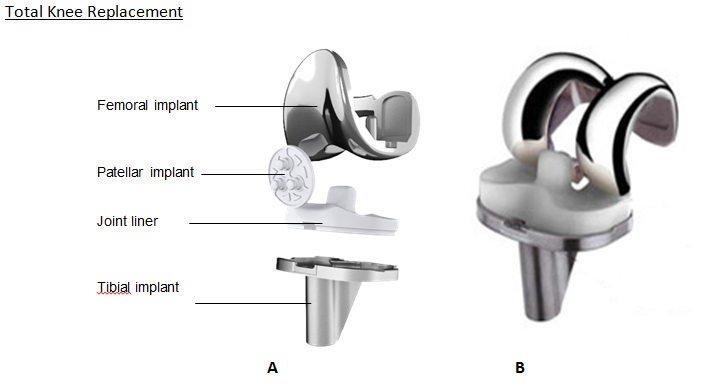
\includegraphics[width=0.7\textwidth]{figures/tka_implant}
\end{center}
\caption{Figuren illustrer en TKA-protese, som består af fire komponenter; et femoralt, patella- og tibialt implantat samt et plastiklag, der placeres mellem det femorale og tibiale implantat og mindsker friktionen. Udformningen af komponenterne gør det muligt at efterligne knæleddets naturlige bevægelse. \citep{robodoc2016}} 
\label{fig:tka_implant1} 
\end{figure}\vspace{-.25cm}

Under operationen ligger patienten på operationsbordet med knæet i en flekteret position. Et snit lægges over patella, hvorefter denne og senerne i leddet eleveres og blotter knæleddet. Hermed får kirurgen adgang til bruskfladerne på femur og tibia. Kirurgen fjerner det ødelagte brusk og en del af knoglen ved hjælp af en guideblok, der skrues ind i femur og sikrer præcis fjernelse af den ønskede mængde væv. Dette gentages på tibia, hvorved der skabes plads til implantaterne, som ses på \figref{fig:tka_implant1}. Midlertidige implantater indsættes for at sikre bevægelsesfriheden er bevaret og testes ved ekstension af knæet. Efterfølgende bores der guidehuller i henholdsvis femur, tibia og patella til fastmontering af de permanente implantater. Fastmonteringen sker ved at dække implantatet og monteringsstedet i bencement, der limer proteserne fast til den eksisterende knoglestruktur. Herefter sikres igen, at bevægelsesgraden er bibeholdt, førend indsnittet lukkes og operationen er fuldendt. En TKA-operation varer typisk omkring én time, hvorefter patienten kan støtte på benet den følgende dag. Efter operationen følger et rehabiliteringsforløb for at støtte og styrke muskulaturen omkring knæet. \citep{Sanna2013} \citep{tka-technique}

Ifølge Sundhedsstyrelsens vurdering er TKA-operationen en effektiv behandling til at øge patientens livskvalitet ved at mindske smerte og øge patientens funktionalitet. Holdbarheden af knæimplantaterne vurderes ud fra antallet af implantater, der er udskiftet efter 10 år, hvor det er påvist, at 90 til 95~\% af implantaterne ikke er revideret. Det er ikke den reelle holdbarhed af den enkelte protese, da flertallet af patienterne dør med et velfungerende implantat. \citep{brostrom2012}

\subsubsection{Kriterier for veludført TKA-operation}\label{tek_succes}
Kriterierne for succesfuld kirurgisk behandling af knæartrose er ifølge Styringsgruppen for Dansk Knæalloplastikregister (DKA) opdelt i fem kriterier. \citep{aarsrapport2016} Disse kriterier er opgivet i tabel \ref{succeskriterier}, hvor standard og landsgennemsnit for Danmark ligeledes er opgivet. 
%, som alle bygger revisionsraten. Altså patienter som har behov for en yderligere knæ operation.

\begin{table}[H]
\centering
\resizebox{\textwidth}{!}{%
\begin{tabular}{ccc}
\rowcolor[HTML]{C0C0C0} 
                                                                                                                                        & \begin{tabular}[c]{@{}c@{}}Standard\\{[}maximale \%{]}\end{tabular} & Landsgennemsnit (Spredning) {[}\%{]} \\ \hline
Andel af patienter med primær TKA på baggrund af primær artrose, \\ som, uanset diagnose, genindlægges indenfor 30 dage efter udskrivning. & 10                                                                                  & \begin{tabular}[c]{@{}c@{}}7,3 \\ (5,8 til 9,5)\end{tabular} \\
Andel af patienter med primær TKA der er revideret indenfor et år.                                                                      & 3                                                                                   & \begin{tabular}[c]{@{}c@{}}1,8 \\ (0,8 til 2,4)\end{tabular} \\
Andel af patienter med primær TKA der er revideret indenfor to år.                                                                      & 5                                                                                   & \begin{tabular}[c]{@{}c@{}}3,3\\ (1,7 til 4,8)\end{tabular}  \\
Andel af patienter med primær TKA der er revideret indenfor fem år.                                                                     & 8                                                                                   & \begin{tabular}[c]{@{}c@{}}6\\ (4,2 til 6,7)\end{tabular}    \\
Andel af patienter, der dør indenfor 90 dage efter primær TKA.                                                                          & 1                                                                                   & \begin{tabular}[c]{@{}c@{}}0,4\\ (0 til 0,7)\end{tabular}    \\ \hline
\end{tabular}%
}
\caption{Tabellen viser succeskriterierne for knæalloplastikoperationer med en standardiseret grænse sammenholdt med landsgennemsnittet. Spredning er indikeret i parentes. Tabellen er modificeret fra \cite{aarsrapport2016}}
\label{succeskriterier}
\end{table}

Det fremgår af \tabref{succeskriterier}, at der i hele Danmark udføres knæalloplastikker, som alle overholder retningslinjerne for behandlingskvaliteten \citep{aarsrapport2016}. 
På trods af at alle operationer overholder de opstillede kriterier, har en betydelig procentdel af patienterne kroniske postoperative smerter. \citep{Bourne2010} Hermed opfyldes succeskriterierne opstillet af DKA, hvormed næsten alle knæalloplastikker kan anses som værende succesfulde. Dette er imidlertid modstridende med andelen af operationer, der er tilfredsstillende ud fra et patientsynspunkt. Det er således væsentligt at identificere eventuelle præoperative risikofaktorer for udvikling af kroniske smerter efter en TKA-operation.  

Et studie af \citer{Lewis2015} har undersøgt prædikatorer associeret med kroniske postoperative smerter ved TKA-operationer. Det blev fundet, at katastrofetænkning, mentalt helbred, smerte forud for operationen og smerte andre steder var de største risikofaktorer for kroniske smerter efter en TKA-operation. 

\subsubsection{Postoperative TKA-resultater} \label{patientermedsmerter}
I 2014 blev der udført cirka 8.800 TKA-operationer, hvoraf 1,8~\% af disse var revisioner et år efter primæroperationen. \citep{aarsrapport2016} Et studie af \citer{Petersen2015} viste, at 19~\% af patienterne efter en primær TKA-operation havde svære til uudholdelige smerter. Det samme var gældende for 47~\% af patienterne, der fik en revision. Et review af \citer{Beswick2012} viste, på baggrund af analyse af tidligere udførte studier, at andelen af patienter med kroniske postoperative smerter et år efter TKA-operation var i intervallet 10 til 34~\%.\\
Et studie af \citer{Petersen2015} viste, at 11~\% af patienterne med primær TKA-operation og 25~\% af patienterne med revisionsoperationen ikke var tilfredse med operationen. \citep{Petersen2015}
\citer{Sakellariou2016} har også undersøgt, hvor stor en andel af patienter, der oplever kroniske postoperative smerter efter en TKA-operation. Ud fra resultaterne viste \citer{Sakellariou2016}, at op mod 39~\% af studiets patienter oplevede moderat til alvorlig smerte et år efter TKA-operationen, imens kun 19~\% af patienterne var utilfredse med resultatet af operationen.\\
Herved antydes en skævhed i forholdet mellem patienter med smerter og utilfredse patienter. Denne observation understøttes af et studie udført af \citer{Jacobs2014}. I studiet blev det påvist, at utilfredsheden i det fleste tilfælde var relateret til enten passiv fleksion, smerte eller funktionsnedsættelse. Der blev foretaget præoperative tests, der indikerede, at der ikke var signifikant forskel på smerte og funktion blandt patienterne, der efter operationen var henholdsvis tilfredse og utilfredse. Efter operationen blev der foretaget en tilsvarende test af de enkelte forsøgspersoner, der viste, at de patienter, som var utilfredse med operationen, havde signifikant dårligere testresultater indenfor de tre nævnte parametre. \citep{Jacobs2014} 
Resultaterne fra et studie af \citer{Bourne2010} indikerer ligeledes, at der er andre parametre end smerte forbundet med utilfredshed efter en TKA-operation; de utilfredse patienter havde, udover signifikant flere smerter, også ledstivhed samt nedsat funktion et år efter operationen, sammenholdt med gruppen af tilfredse patienter. Studiet indikerede ligeledes, at den største prædiktor for utilfredshed efter en TKA-operation er, at patientens egne forventninger til operationensresultatet ikke bliver indfriet. Derfor kan der ikke sættes lighedstegn imellem patienters oplevede smerter og deres tilfredshed.


%
%(1) http://www.robodoc.com/patient_about_faqs.html
%
%(2) https://www.youtube.com/watch?v=tKji04oFGdU

% (3) http://www.ortopaedi.dk/fileadmin/Guidelines/Referenceprogrammer/Osteotomi_og_TKA.pdf

	%(4) Surgical approaches in total knee arthroplasty.
	
%	(5) tka-technique
%
%(79) Dahl AW, Toksvig-Larsen S, Roos EM. A 2-year prospective study of patient- relevant outcomes in patients operated on for knee osteoarthritis with tibial osteot- omy. BMC Musculoskeletal Disorders 2005;6(1):18. Er lagt på mendlay
%(80) Hoell S, Suttmoeller J, Stoll V, Fuchs S, Gosheger G. The high tibial osteoto- my, open versus closed wedge, a comparison of methods in 108 patients. Arch Or- thop Trauma Surg 2005;125(9):638-643. Er lagt på mendelay

%Når de non-kirurgiske behandlingsmuligheder ikke har kunne løse patienten fra smerter, er kirurgi det næste skridt i behandlingsforløbet. Der findes flere behandlingsmuligheder inden for kirurgiskbehandling af knæartrose, dog med TKA som den endelige udvej. %Valget af operation og typen af den afhænger af flere faktorer, blandt andet patients alder, aktivitetsniveau og hvor fremskreden artrosen er.


%\subsubsection{Osteotomi}
%Ved degenerative forandringer i knæleddet, grundet primær eller postttrumatisk knæledsarterose, kan patienter opleve belastningsreleaterede smerter, hvilket blandt andet kan skyldes fejlstilling. Osteotomi har tilformål at afhjælpe den mekaniske belastning i det berørte område, for derved at afhjælpe smerterne. Ved osteotomi fjernes der oftest en kile af tibia-knoglen og det resterende knogle sikres med skruer og metal plader. Proceduren ændre knæets mekaniske akse, hvilket vil ændre belastningen af de degenererede områder. \citep{Osteotomi_og_TKA} Ved yngre (<50år) og aktive patienter vil der være større sandsynelighed for at tilbyde osteotomi frem for den mere invasive TKA, derfor anbefales osteotomi af sundhedstyrelsen til behandling af mildere former for artrose med fejlstilling \citep{Osteotomi_og_TKA} \citep{brostrom2012}. Behandlingen ses som en midlertidig behandling der kan udskyde behovet for TKA. Ifølge et kohordestudie kan der forventes en smertelindring hos 80\%~ af patienterne der får udført osteotomi. \textbf{rigtige kilder tak!(79)(80)} Ifølge \cite{brostrom2012} må det forventes at 30 til 50\%~ af patienterne der får foretaget en osteotomi, senere vil få behov for en alloplastik operation. \citep{brostrom2012} Tilbagevendende smerter korreleres til tab af korrektionen, samt progression af artrosen. Får patienten således svære smerte igen, kan en TKA komme til overvejelse \citep{Osteotomi_og_TKA}. 
% \textbf{Der er data på mere specifikke tilfredsheds undersøgelser, men ser ikke nogen trund til at medtage dem. }